%
%  untitled
%
%  Created by Hendrik Strobelt on 2012-07-09.
%  Copyright (c) 2012 . All rights reserved.
%
\documentclass[a4paper, twocolumn,
final
%draft
]{article}

\usepackage[top=1.5cm,bottom=2cm,left=1.5cm,right=1.5cm]{geometry}

\usepackage{url}
\usepackage{microtype}
\pagestyle{empty}

% Use utf-8 encoding for foreign characters
\usepackage[utf8]{inputenc}
\usepackage[T1]{fontenc}

% Setup for fullpage use
%\usepackage{fullpage}
\usepackage[ngerman,british, english]{babel}
% Uncomment some of the following if you use the features
%
% Running Headers and footers
\usepackage{fancyhdr}

% Multipart figures
\usepackage{subfigure}

% More symbols
%\usepackage{amsmath}
%\usepackage{amssymb}
%\usepackage{latexsym}

% Surround parts of graphics with box
\usepackage{boxedminipage}

% Package for including code in the document
\usepackage{listings}

% If you want to generate a toc for each chapter (use with book)
\usepackage{minitoc}

% This is now the recommended way for checking for PDFLaTeX:
\usepackage{ifpdf}

\ifpdf
\usepackage[pdftex]{graphicx}
\else
\usepackage{graphicx}
\fi


\title{BusVis -- Interactive Visualization of a Public Transport System}
\author{Feeras Al-Masoudi, Josua Krause,  Marc Spicker, and Leonard Wörteler  }

\date{\today}


\begin{document}
\selectlanguage{english}

\maketitle
\thispagestyle{empty}

\section*{Introduction}
We present \textsc{BusVis}, a tool for explorative analysis that is capable of visualizing
transportation systems, illustrated on the bus system of Konstanz.
The focus on a specific station is chosen interactively by the user. The visualization adapts to the selection by transforming the overview into a locally correct projection w.r.t. distances to neighbours while preserving geographical context.

\begin{figure}[h]
	\centering
	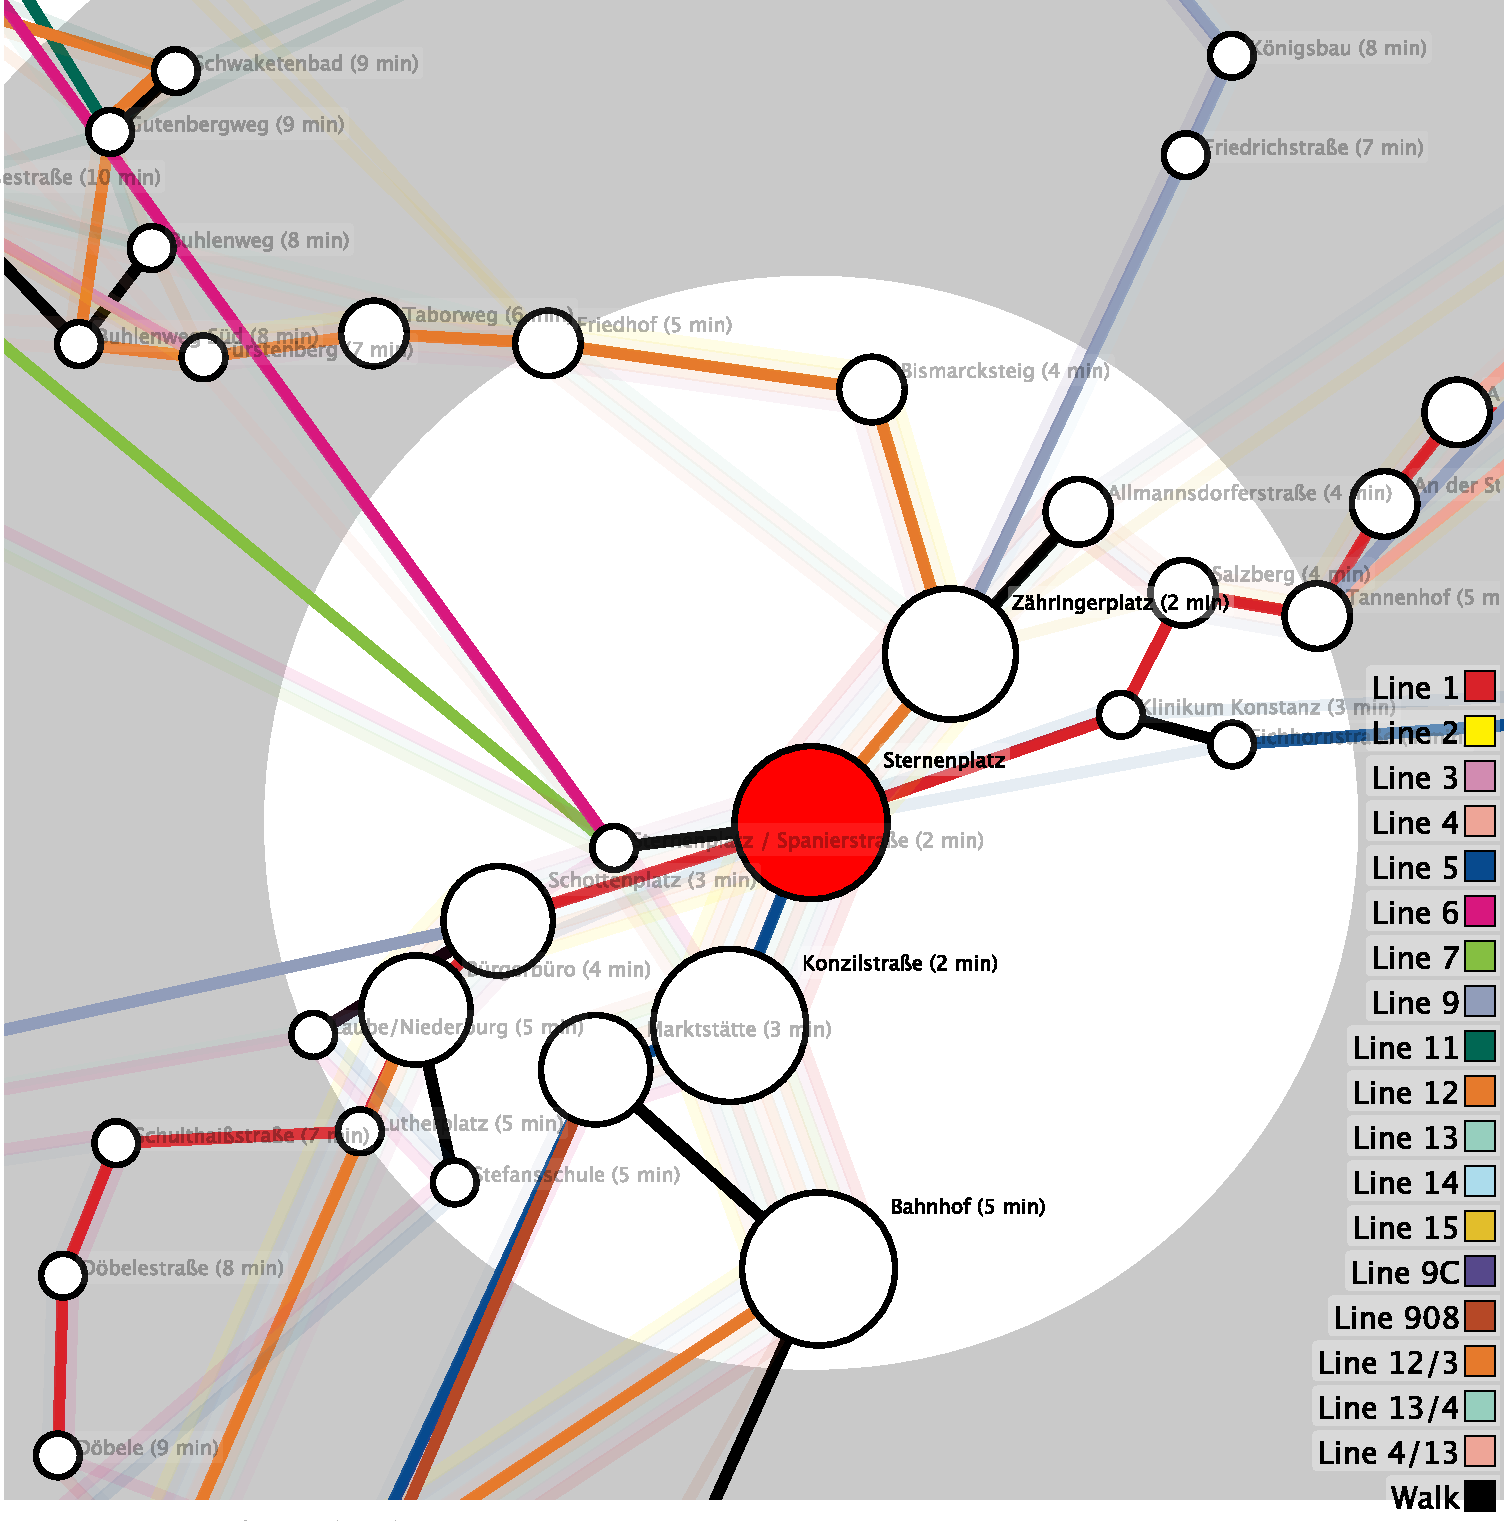
\includegraphics[width=0.9\linewidth]{svgs/teaser.pdf}
\end{figure}

\section*{Dataset and Preprocessing}

The data consists of 123 bus stations, 18 bus lines, schematic and geographic positions for each stop, walking distances, and 16,088 time-dependent directed edges.
% As a first step data format has been changed from \texttt{XLS} to \texttt{CSV} format in order to parse it more easily. 
The following data pre-processing steps were applied:
\begin{description}
\setlength{\itemsep}{0pt}
\item[Cleaning.] Data files were converted from \texttt{XLS} to \texttt{CSV} and missing values in the time table 
  were added.
\item[Walking distances.] We then added walking distances between each station the enrich the data and allow the
application to incorporate that users would probably walk small distances instead of waiting for a bus.
\item[Schematic plan positions.]
 We annotated each bus station with its corresponding position on the schematic map.
\end{description}

\section*{Visualization}

We show the travel distances from a selected source to all destinations in one visualization.
The stations are represented as nodes and their connections as edges in a \emph{node-link diagram}.
We encode travel times by visual distances. Two alternative layouts allow either local correctness or global stress minimization for the described distance mapping.

%Because multiple bus lines may drive between two stations, the edges which represent the bus lines
%are drawn next to each other with the color indicating the line number. Initially the position of the nodes
%corresponds to the geographic position of the stations. The user can select a source station 
%and one or more destination stations and the visualization will then highlight edges between the source
%and the destinations, while providing interactions of a \emph{ZUI}, i.e. zooming and panning. The main
%visualization can be toggled between a radial layout and stress-based layout which both have their pros and cons.
 
\begin{description}
\setlength{\itemsep}{0pt}
\item[Radial Layout.]  The source is the center of the layout. Destinations are positioned in a way that the distance to the center is an exact mapping of the source-destination time distance.
To preserve the mental map we chose the angle between two stations w.r.t. the source to align with geographic directions. Concentric rings represent five-minute intervals.
\begin{figure}[h]
	\centering
		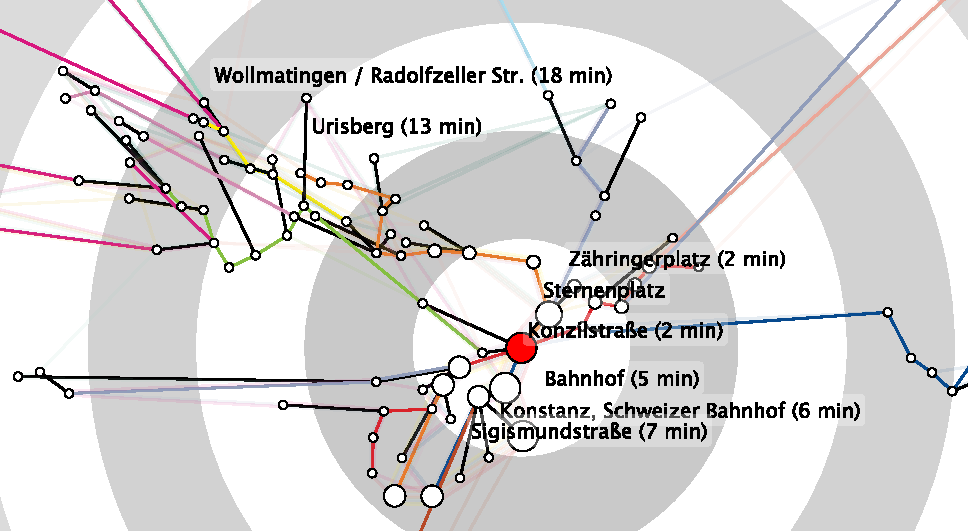
\includegraphics[width=0.9\linewidth]{svgs/radial_crop.pdf}
\end{figure} 
\item[Stress-Majorization Layout.]  This layout projects travel times between adjacent bus stations to length of edges by minimizing a global stress function. We used the \emph{SMACOF}\footnote{Scaling by Majorizing A COnvex Function} algorithm as an efficient solver.
The geographic positions of the stations are chosen as initial layout in order to roughly preserve the shape of the bus network. This works well because travel time increases with geographical distance.
\begin{figure}[h]
	\centering
		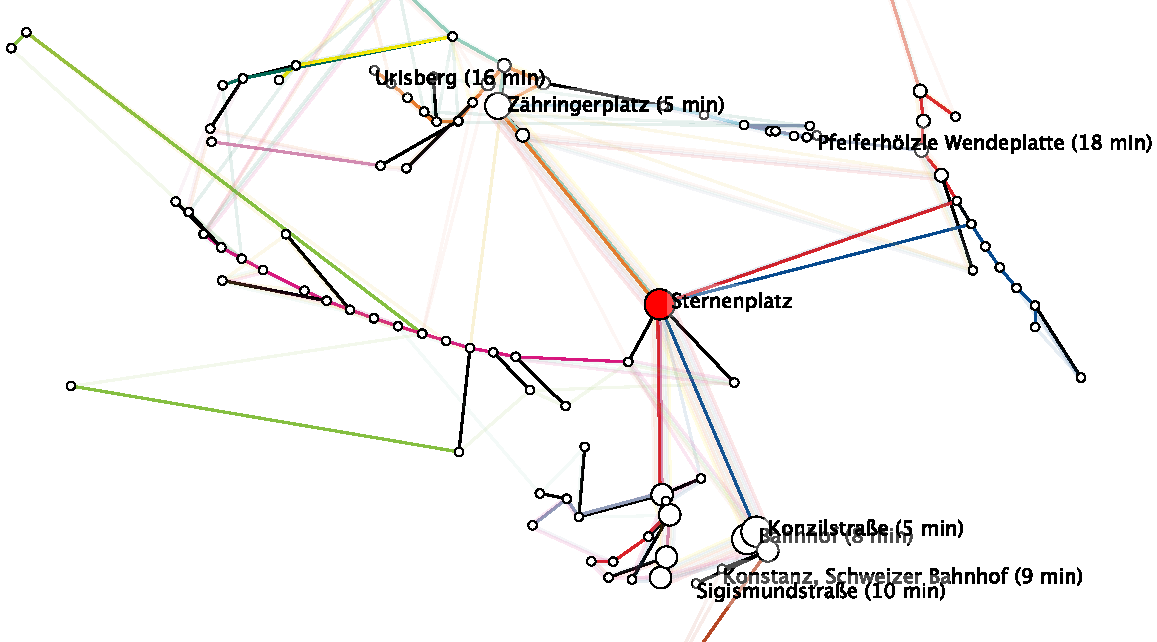
\includegraphics[width=0.9\linewidth]{svgs/stress_crop.pdf}
\end{figure} 
\end{description}

\section*{Tool}
Our tool is implemented in Java and provides a GUI to interact with and configure the visualization.
Initially the nodes are located at their geographic positions. The user can select a station as source.
Then the shortest routes to all other stations are calculated and the layout changes accordingly.
Transitions are smoothly animated to retain the mental map.
Additionally one or more destinations can be selected and the visualization will then highlight the corresponding routes. The user can switch between radial and stress layout.

The tool includes a schematic overview
which allows the user to select bus stations even when the main visualization has changed.
The user interface allows to modify parameters of the routing algorithm, e.g. the 
current time, the maximal allowed walking time, or minimal stopover time.
A real-time and fast-forward mode can be enabled to simulate bus tracking at different speed.

\section*{Use Cases}
A bus plan is very difficult to read when source and destination are not connected by
the same bus line. Normally a simple routing application can be used to find the fastest
route to a given destination. However this only works with one source and one destination. Our
visualization shows shortest routes to all bus stations in a network from a single source.
\begin{description}
\item[Comparing travel times.]
The bus stations \emph{Universität} and \emph{Egg} for example are very close. This raises the question when it is rewarding to chose one destination over the other. Our visualization gives a simple advice by just choosing
the station that is nearer to the center (Figure \ref{fig:cmp}).

\begin{figure}[h!]
	\centering
	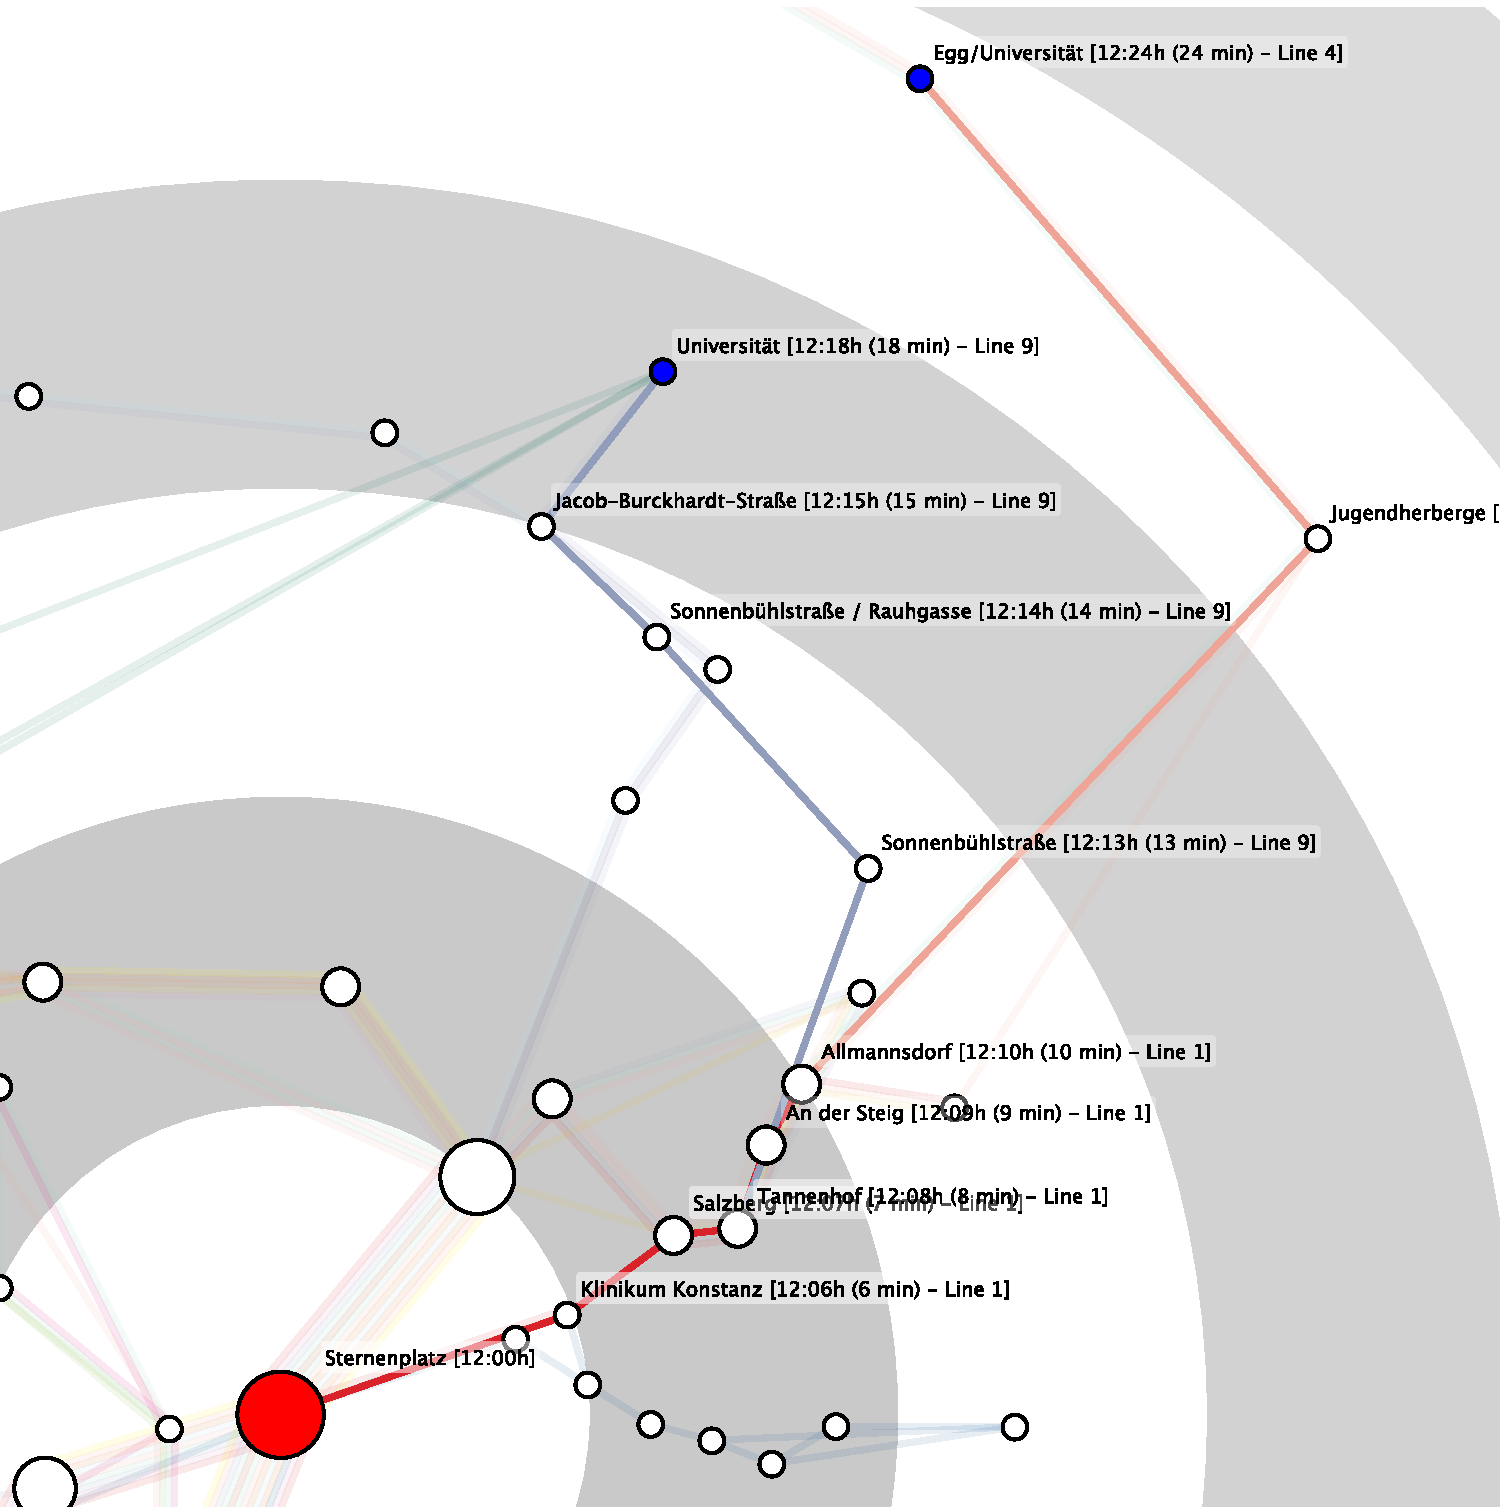
\includegraphics[width=0.4\linewidth]{svgs/routes_0.pdf}
	\hspace{1em}
	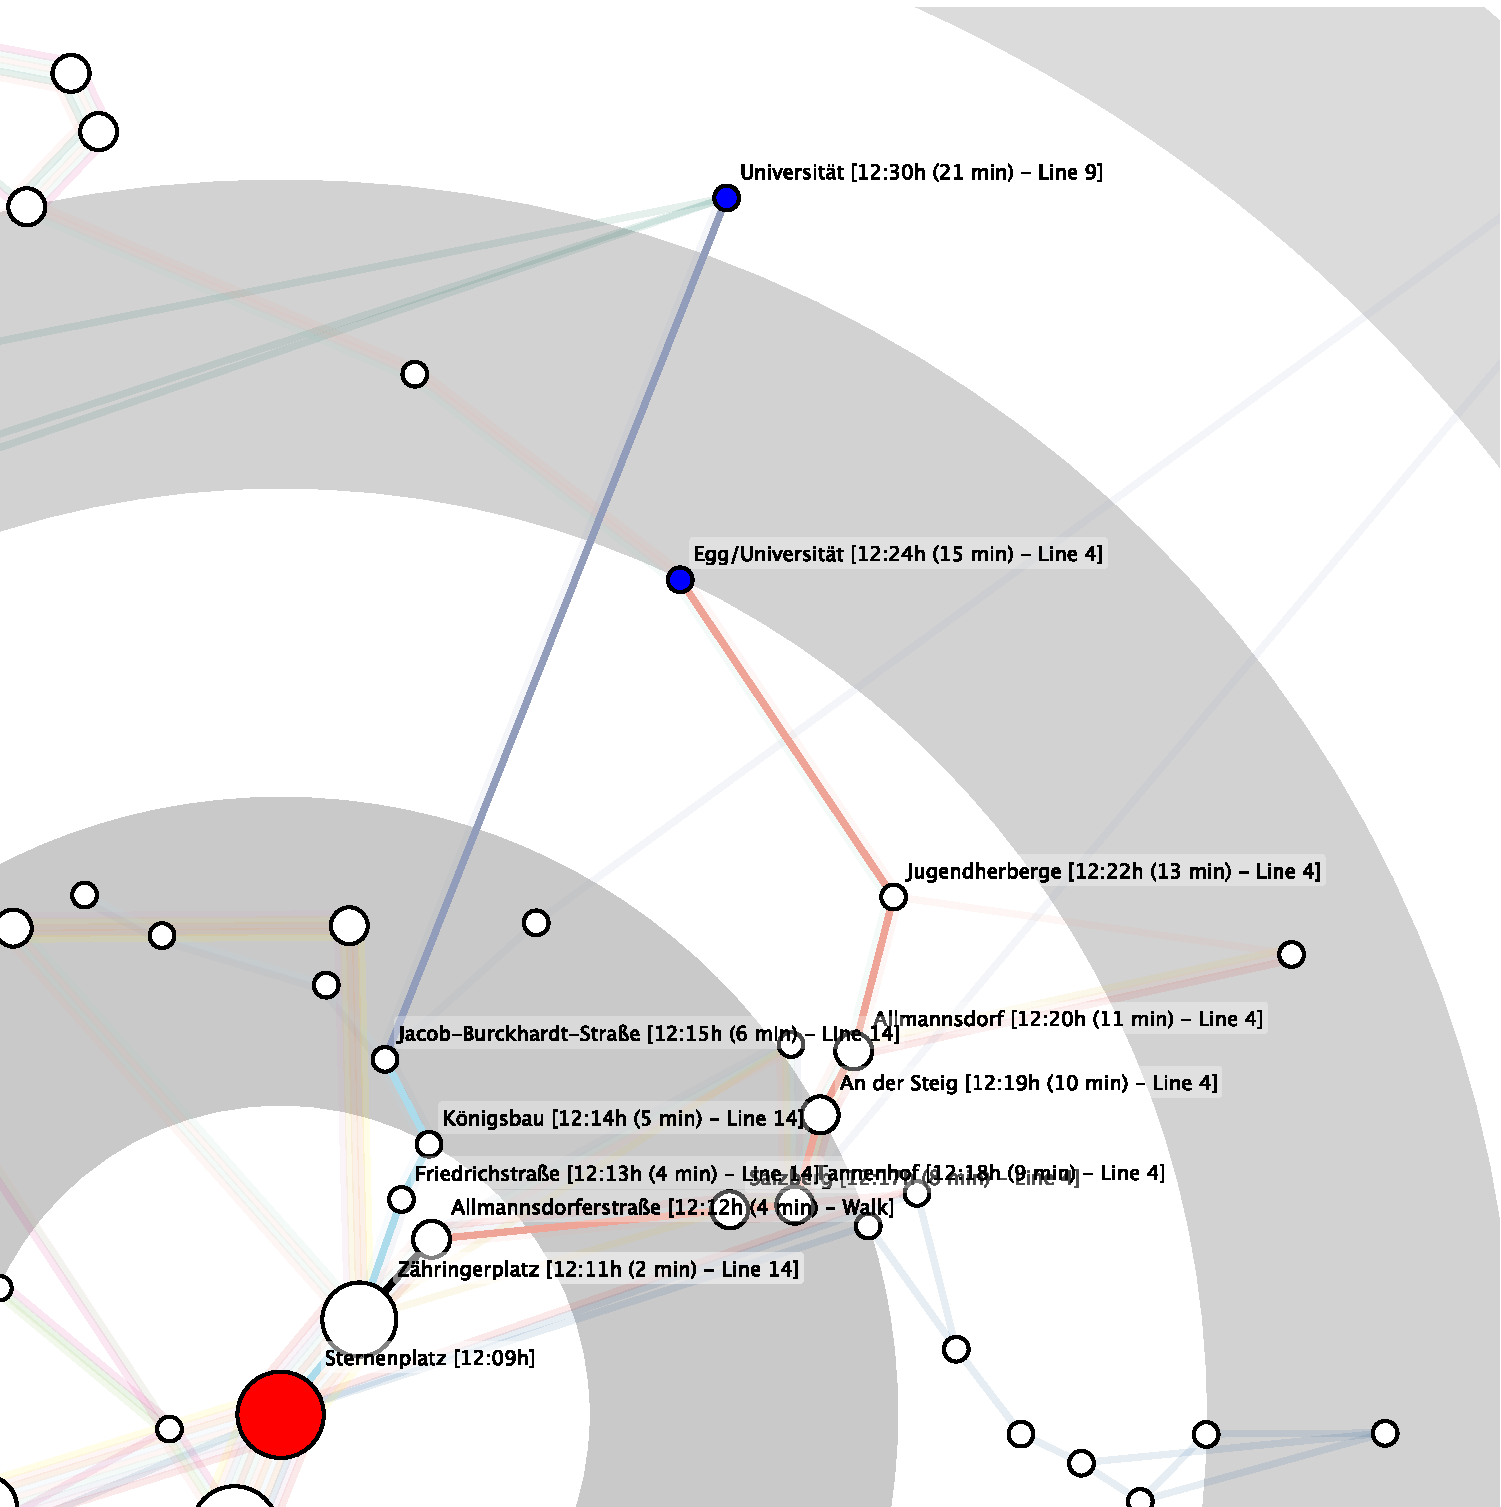
\includegraphics[width=0.4\linewidth]{svgs/routes_1.pdf}
	\caption{Routes from \emph{Sternenplatz} (red) to
	\emph{Universität} and \emph{Egg} (both blue) at different times.
	On the left \emph{Universität} is nearer than \emph{Egg} and on the
	right vice versa.
	}
	\label{fig:cmp}
\end{figure}
\item[Finding weakly connected stations.]
The possibility to change the starting time of a path helps to analyse the reachability of bus
stations over time. For example frequent walk suggestions indicate a bad reachability of a bus
station, as seen in Figure \ref{fig:walk}.
\begin{figure}
	\centering
	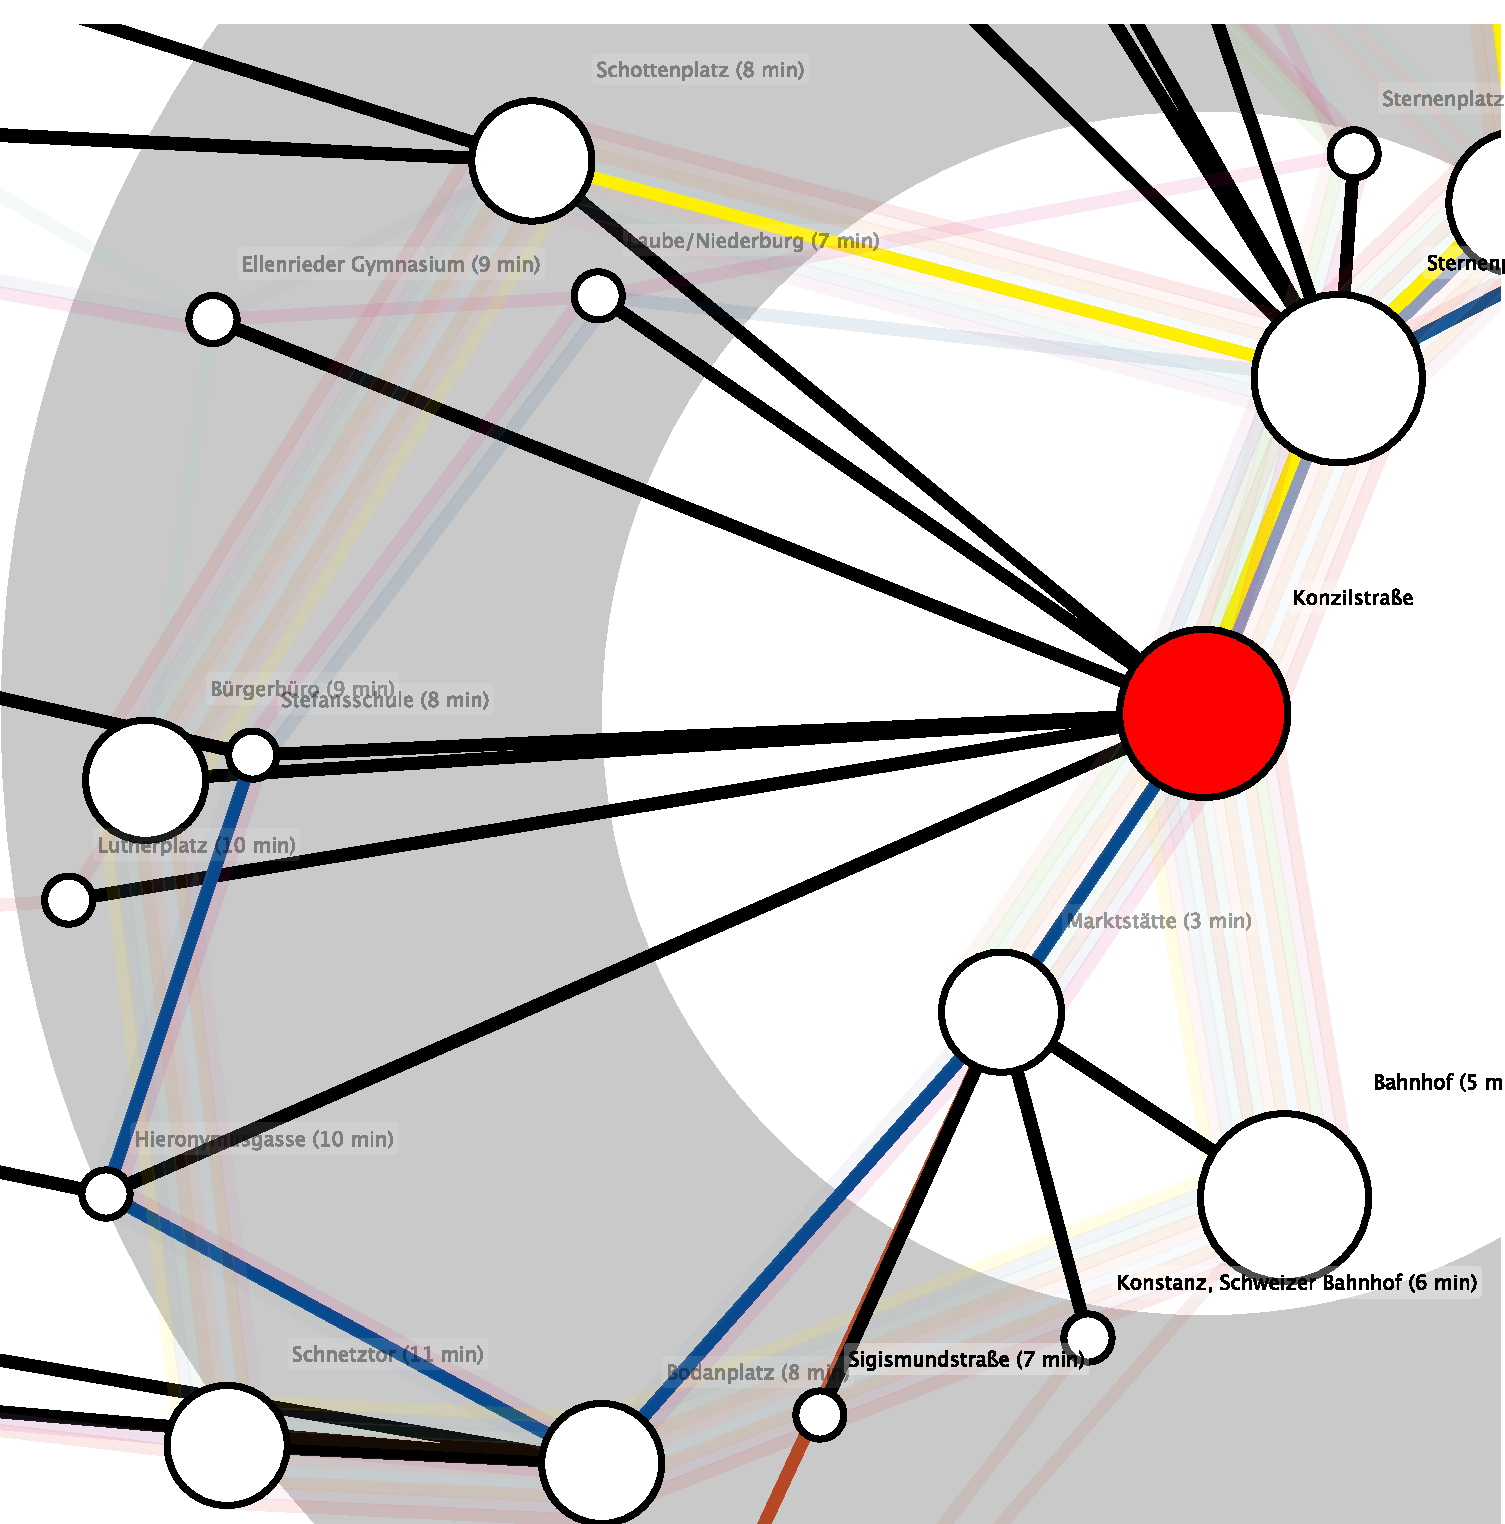
\includegraphics[width=0.4\linewidth]{svgs/edges.pdf}
	\caption{Black edges indicate walks.
	Sometimes it is better to walk from \emph{Konzilstraße}.
	}
	\label{fig:walk}
\end{figure}
\end{description}

\section*{Challenges}

\begin{description}
\item[Routing.] Obligatory stopover times violate invariants of classical routing algorithms, as
  suboptimal intermediate steps can still lead to an optimal route.
  
  We adapted our algorithm accordingly.
  Resulting performance problems were solved by excluding suboptimal routes earlier.
\item[Overlaps.] We resolved overlaps in the radial layout by changing the angle of the nodes without
compromising the correctness of the visualization. This is not possible in the stress-majorization layout.
\item[Drawbacks of the layouts.] In the radial layout, it is very easy to misinterpret the distance
between two nodes: If they do not lie on a line from the center, their distance has no meaning,
because only the difference between their distances to the center is meaningful. For this reason we
introduced the additional stress-majorizing layout. Every edge tries to have the length which is
proportional to the time it takes to traverse this edge. However, this is an optimization problem
which does not result in a exact solution. 
\end{description}

\section*{Conclusion}

We provided a tool to visualize shortest routes in a transportation network which, in contrast to
standard techniques like bus plans, allows the user to quickly explore transportation schedules.
Real-time interaction enables the user to navigate in the visualization and modify parameters
with instant feedback. The tool can be used to compare travel times to different stations at
different times and find flaws in the schedule.

\section*{Authors' Contributions}

\begin{description}
\setlength{\itemsep}{0pt}
  \item[Feeras Al-Masoudi] Labels, fast-forward animations.
  \item[Josua Krause] Radial layout, user interaction.
  \item[Marc Spicker] Overview, edge drawing, GUI.
  \item[Leonard Wörteler] Stress-majorization layout, routing.
\end{description}

\section*{References}

\begin{description}
\item[Tom Carden.] "Travel Time Tube Map"

  \url{http://www.tom-carden.co.uk/p5/tube_map_travel_times/applet/}
\item[J. de Leeuw.] "Applications of convex analysis to multidimensional scaling."
\item[Misue et al.] "Layout Adjustment and the Mental Map"
\end{description}

\end{document}
